
Through its effect on drift velocity, recombination, and lifetime, the \efield is a critical parameter for physics signals as it ultimately affects the spatial resolution and energy response of the detector. The primary purpose of a laser system is to provide an independent, fine-grained estimate of the \efield in space and time.
It would be extremely valuable to achieve measurements of electron lifetime with the laser system, but the feasibility of that is still under discussion. %and will be the goal of dedicated R\&D in the validation plan. 
The R\&D plan in \dword{protodune2} will address the feasibility of carrying out charge-based measurements which, if successful, would open up the possibility of using the laser to measure electron lifetime. So, except where specifically indicated, the rest of this section will focus on 
%be concerned with the 
drift velocity and \efield measurement.

\subsubsection{Physics Motivation}
Because it measures spatial distortions of straight tracks, the laser system actually measures the local drift velocity field directly and helps define the detector \dword{fv}, and this in itself is an important input for the \dword{lbl} analysis. 
%, and this is in itself an input to the analysis.
%Still,
However, it is still important to use information independent of the charge in order to disentangle effects like lifetime and recombination from \efield distortions. The laser system can do this, by using the position information to derive the \efield from the local velocity map, taking into account the colinearity between both vectors, and the relatively well studied relation between the magnitude of the drift velocity and the \efield, considering a temperature dependence (see~\cite{Li:2015rqa} and references [29, 45-58] therein). A laser system also has the intrinsic advantage of being immune to recombination effects, thus eliminating particle-dependent effects.  

Several sources may distort the \efield temporally  and/or spatially in the detector. Current simulation studies indicate that positive ion accumulation and drift (space charge) due to ionization sources such as cosmic rays or \Ar39 is small in the \dword{dune} \dword{fd}, causing \efield distortions of at most \SI{0.1}{\%}~\cite{bib:mooney2018}.
However, not enough is known yet about the fluid flow pattern in the \dword{fd} to exclude the possibility of stable eddies that may amplify the effect for both \single and \dual modules. %\dword{spmod} and \dword{dpmod}. 
This effect can be further amplified significantly in the \dword{dpmod} due to accumulation in the liquid of ions created by the electron multiplication process in the gas phase.
%due to ion accumulation at the liquid-gas interface. 
Additionally, other sources in the detector (especially detector imperfections) can cause \efield distortions. For example, \dword{fc} resistor failures, non-uniform resistivity in the voltage dividers, \dword{cpa} misalignment, \dword{cpa} structural deformations, and \dword{apa} and \dword{cpa} offsets and  deviations from flatness can create localized \efield distortions. These effects are presented in Figures~\ref{fig:efield_cpa_distortions_boyu2017} and \ref{fig:efield_resistorfailure_mooney2019}, showing the effect of a few \% on the \efield from \SI{2}{\cm} \dword{cpa} position tilts and %of 
up to \SI{4}{\%} from \dword{fc} single resistor failures.

\begin{dunefigure}[Impact on \efield of \dshort{cpa} position distortions]{fig:efield_cpa_distortions_boyu2017}
{Illustration of a possible distortion of the \dword{cpa} position~\cite{bib:yu2017a}, assuming a \SI{2}{\cm} swing, and its impact on \efield (right).}
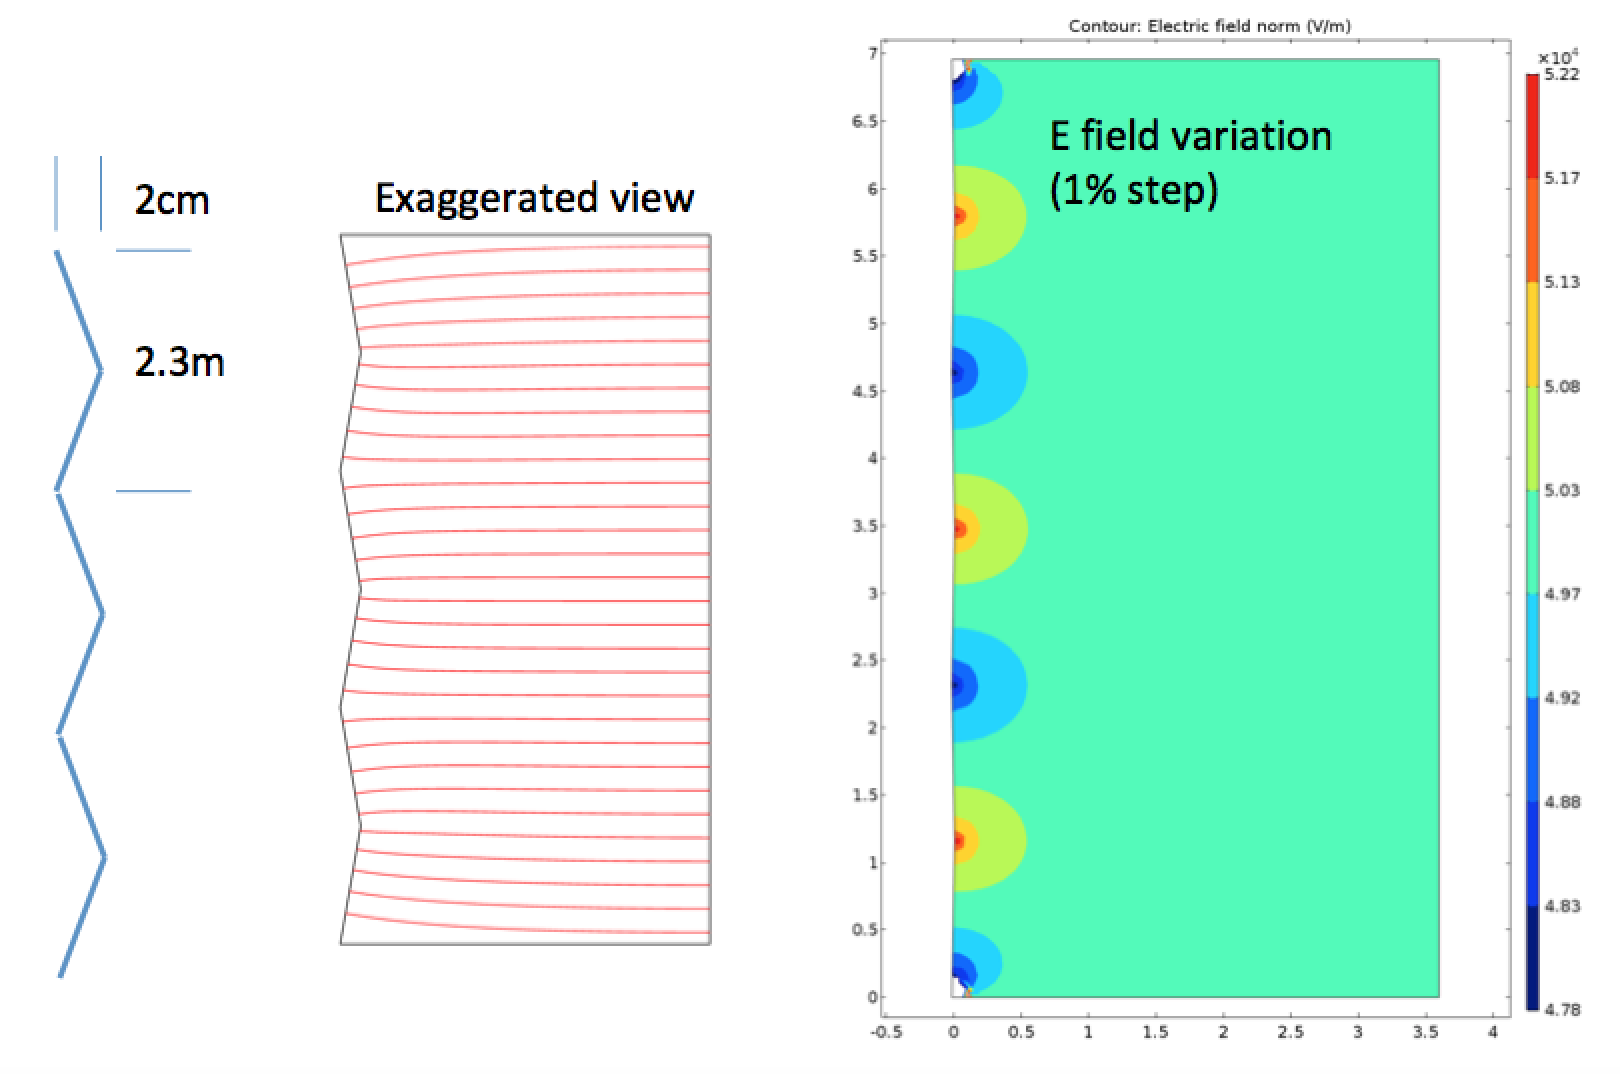
\includegraphics[width=0.8\textwidth]{efield_cpa_distortions_boyu2017.png}
\end{dunefigure}

\begin{dunefigure}[Impact on \efield of \dshort{fc} resistor failures]{fig:efield_resistorfailure_mooney2019}
{Impact on \efield magnitude distortions of a single \dword{fc} resistor failure~\cite{bib:mooney2019a}.}
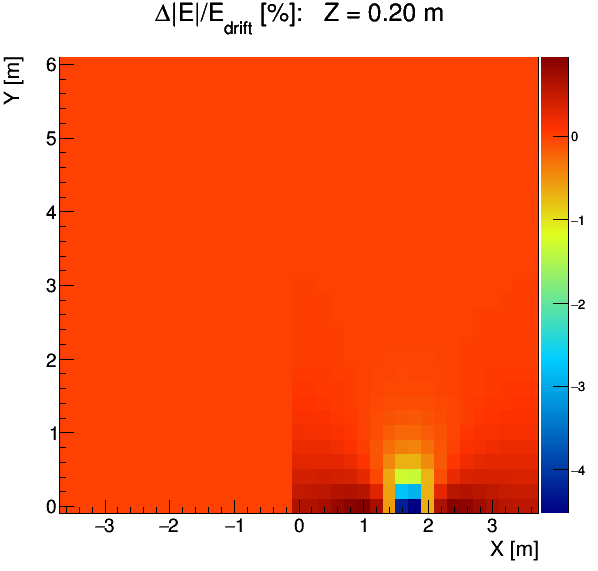
\includegraphics[width=0.5\textwidth]{efield_resistorfailure_mooney2019.png}
\end{dunefigure}

In both \single and \dual modules, %\dword{spmod} and \dword{dpmod} systems, 
a resistor failure will create significant, local \efield distortions that must be identified. In the \dword{dpmod}, %system, 
four resistors would have to fail to cause a failure across the \dword{fc} gap, but even one failure in the \dword{spmod} can have an effect; this may be partly, but not completely, mitigated by modifying the \dword{hv}. While the resistor failure will be detected temporally, its location in space is not possible to determine from slow controls monitoring data. Misalignments of detector objects or deformations may also create \efield distortions; while individual effects may be small, it is possible to have a combined, significant effect.
Each individual \efield distortion may add in quadrature with other effects, and can aggregate up to \SI{4}{\%} under certain conditions. Understanding all these effects requires in situ  measurement of \efield for proper calibration. 

Useful secondary uses of laser include alignment (especially modes that are weakly constrained by cosmic rays),
%; see Figure~\ref{fig:apacurtainalign}),
stability monitoring, and diagnosing detector performance issues
%failures 
(e.g., \dword{hv}).  
Misalignment may include physical deformation and/or rotations of objects within the detector. Given the expected low rate of cosmic ray events (about 3500/day/10-kt) at the underground location, calibration with cosmic rays is not possible over short time scales. Even over long time scales, certain alignment directions  are difficult to assess with cosmic rays alone, such as distortions of the detector that preserve the gap widths and do not shift the \dwords{apa} in $x$ near the gaps relative to one another.
These distortions include global shifts and rotations in the locations of all detector elements, and crumpling modes where the edges of the \dwords{apa} hold together but angles are slightly different from nominal.   

%\fixme{SG: Can you check if you agree with this text below?}
With respect to electron lifetime, the preliminary results from \dword{pdsp} purity monitors and cosmic ray analyses indicate significant variations with time and space, both between monitors at different vertical coordinates (see \dword{tdr} \spchcisc), and between the regions inside and outside the \dword{tpc}. The possibility of carrying out such measurements with the ionization laser is therefore quite interesting. The ArgonTUBE experiment obtained lifetime measurements with laser~\cite{Ereditato:2013xaa} compatible with the cosmic ray ones, but it is not clear yet if this is possible at very large scales, since the modelling of the density of ionization charge created along the tracks presents challenges related to the previously mentioned self-focusing. Therefore the characterization of the ionization charge density from laser tracks will be an important goal of the development plan in \dword{protodune2}.


%A laser system also has the intrinsic advantage of being immune to recombination, thus eliminating particle-dependent effects.  





%%%%%%%%%%%%%%%%%%%%%%%%%%%%
\subsubsection{Requirements}
\label{sec:sp-calib-laser-req}



The energy and position reconstruction requirements for physics measurements lead to requirements on the necessary precision of the laser %calibration 
\efield measurement, its spatial coverage and granularity. The next sections discuss the rationale behind each requirement, which we take as the \dword{dune} specification.
%, with ALARA (or AHARA for the coverage) as goal.

\paragraph{\efield precision:}


In the \dword{lbl} and high-energy range, \physchlbl of this \dword{tdr}
%the \dword{dune} physics \dword{tdr} 
states that the calibration information must provide approximately \num{1} to \SI{2}{\%} understanding of normalization, energy scale and resolution, and position resolution within the detector.
Because a smaller \efield leads to higher electron-ion recombination and therefore a lower collected charge, distortions of the \efield can introduce
%are one of the possible causes of an 
energy scale bias. To connect this
%that requirement 
to a specification for the necessary precision of the \efield measurement, we note that, via recombination studies~\cite{bib:mooney2018}, we expect a \SI{1}{\%} distortion on \efield to lead to a \SI{0.3}{\%} bias on collected charge.
Because other effects will contribute to the lepton energy scale uncertainty budget, we consider a goal for the 
%calibration 
laser system to measure the \efield to a precision of $\sim$\SI{1}{\%} so that its effect on the collected charge is well below \SI{1}{\%}.
This is also motivated by consistency with the high level DUNE specification on field uniformity throughout the volume due to component alignment and \dword{hv} system, that 
%was 
is set at \SI{1}{\%}.
Together with two other high-level \dword{dune} specifications, the \dword{apa} wire spacing (\SI{4.7}{\mm}) and the front end peaking time (\SI{1}{\micro\s}), the effect of this \efield precision requirement on engineering parameters of the calibration laser system is discussed further %ahead, 
in Section~\ref{sec:sp-calib-sys-las-ion-meas}.

\paragraph{\efield measurement coverage:}

In practice, measuring the \efield  throughout the whole volume of the \dword{tpc} will be difficult, so we must establish a goal for the coverage and granularity of the measurement. 
Until a detailed study of the propagation of the coverage and granularity into a resolution metric is available, a rough estimate of the necessary coverage can be made as follows.

Assuming \SI{4}{\%} as the maximum \efield distortion %resulting 
that is %expectable 
expected from a compounding of multiple possible effects in the \dword{dune} \dword{fd} %as stated in the physics volume of the \dword{tdr},
as described in the previous section,
%(\cite{Abi:2018dnh}, page~4-53), 
we can then ask what would be the maximum acceptable size of the spatial region uncovered by the calibration system, if a distortion of that magnitude (systematically biased in the same direction) were present in that region. Our criterion of acceptability is to keep the overall \efield distortion, averaged over the whole detector, at the \SI{1}{\%} level. 
%, so then that 
To meet this requirement, the aforementioned spatial region should be no larger than \SI{25}{\%} of the total fiducial volume. Therefore, we aim to have a coverage of \SI{75}{\%} or more.

In addition, we need to consider that the method used to estimate \efield distortions is based on obtaining position displacement maps~\cite{bib:uBlaser2019}, and that the comparison between the reconstructed and true direction of a single track does not %univocally  %unequivocally
unambiguously determine a specific displacement map. Having tracks coming from different origins crossing in the same position is a direct way to eliminate that ambiguity, since the displacement vector is given simply by the vector connecting the intersections of the two reconstructed and the two true tracks. A joint iterative analysis of several close-by tracks is the default method for all other positions, but the system design should allow for the maximum possible number of positions %where there can be 
for crossing tracks from different beams.

\paragraph{\efield measurement granularity:}

Volume~\volnumberphysics~(\voltitlephysics) of this \dword{tdr} states that a \dword{fv} uncertainty of \SI{1}{\%} is required. 
This translates to a position uncertainty of \SI{1.5}{\cm} in each coordinate (see Chapter~\ref{ch:fdsp-apa}). 
In the $y$ and $z$ coordinates, position uncertainty is given mainly by the \dword{apa} wire pitch, and since this is about \SI{4.7}{\mm}, the requirement is met. In the drift ($x$) direction, the position is calculated from timing, and considering the electronics peaking time of \fepeaktime, the uncertainty should be even smaller.

The position uncertainty, however, also depends on the \efield, via the drift velocity. Because the position distortions accumulate over the drift path of the electron, it is not enough to specify an uncertainty on the field. We must accompany it by specifying the size of the spatial region of that distortion. For example, a \SI{10}{\%} distortion would not be relevant if it was confined to a \SI{2}{\cm} region and if the rest of the drift region was at nominal field.
%So 
Therefore, what matters is the product of [size of region] $\times$ [distortion]. Moreover, one can distinguish distortions into two types:
\begin{enumerate}
\item Those affecting the magnitude of the field. Then the effect on the drift velocity $v$ is also a change of magnitude. According to the function provided in \cite{Walkowiak:2000wf}, close to \SI{500}{\V\per\cm}, the variation of the velocity with the field is such that a \SI{4}{\%} variation in field $E$ leads to a \SI{1.5}{\%} variation in $v$.
\item Those affecting the direction of the field. Nominally, the field $E$ should be along $x$, so $E = E_L$ (the longitudinal component). If we consider that the distortions introduce a new transverse component $E_T$, in this case, this translates directly into the same effect in the drift velocity, which gains a $v_T$ component, $v_T=v_L  E_T/E_L $, i.e., a \SI{4}{\%} transverse distortion on the field leads to a \SI{4}{\%} transverse distortion on the drift velocity.
\end{enumerate}

Thus, a \SI{1.5}{\cm} shift comes about from a constant \SI{1.5}{\%} distortion in the velocity field over a region of \SI{1}{\m}. In terms of \efield, that could be from a \SI{1.5}{\%} distortion in $E_T$ over \SI{1}{\m} or a \SI{4}{\%} distortion in $E_L$ over the same distance.

%From ref.~\cite{Abi:2018dnh}, page~4-53, 
\efield distortions can be caused by space-charge effects due to accumulation of positive ions caused by \Ar39 decays (cosmic ray rate is low in \dword{fd}), or detector defects, such as \dword{cpa} misalignments (Figure~\ref{fig:efield_cpa_distortions_boyu2017}), \dword{fc} resistor failures (Figure~\ref{fig:efield_resistorfailure_mooney2019}), resistivity non-uniformities, etc.
%~\cite{Abi:2018dnh}. 
These effects added in quadrature can be as high as \SI{4}{\%}. 
%From ref. ~\cite{bib:mooney2018}, 
The space charge effects due to \Ar39~\cite{bib:mooney2018} can be approximately \SI{0.1}{\%} for the \dlong{sp} (\dshort{sp}), and \SI{1}{\%} for the \dshort{dp} (\dlong{dp}), so in practice these levels of 
%that kind of distortion 
distortions must cover several meters to be relevant.
Other effects due to \dword{cpa} or \dword{fc} imperfections can be higher because of space charge, but they are also much more localized. If we assume there are no foreseeable effects that would distort the field more than \SI{4}{\%}, and considering the worst case scenario (transverse distortions), then the smallest region that would produce a \SI{1.5}{\cm} shift is \SI{1.5}{\cm}/\num{0.04}~=~\SI{37.5}{\cm}. This provides a target for the granularity of the measurement of the \efield distortions in $x$ to be smaller than approximately \SI{30}{\cm}, with, of course, a larger region if the distortions are smaller. Given the above considerations, then a voxel size of \num{10}$\times$\num{10}$\times$\SI{10}{\cubic\cm} appears to be enough to measure the \efield with the granularity needed for a good position reconstruction precision. In fact, because the effects that can likely cause bigger \efield distortions are problems or alignments in the \dword{cpa} (or \dword{apa}) or in the \dword{fc}, it is conceivable to have different size voxels for different regions, saving the highest granularity of the probing for the walls/edges of the drift volume.









\subsubsection{Design}
\label{sec:sp-calib-sys-las-ion-des}
%\paragraph{Baseline design}

The design of the laser calibration system for \dword{dune} is largely based on the design of the system built for \dword{microboone}~\cite{microboone}, which in turn was based on several previous developments~\cite{Rossi:2009im,Zeller:2013sva,Ereditato:2014lra,Ereditato:82014tya}. A similar system was also built for \dword{captain}~\cite{Berns:2013usa} and in the near future, will be built for \dword{sbnd}~\cite{Antonello:2015lea}. Operation of the \dword{microboone} system has already taken place. A preliminary report was given in~\cite{bib:chen2018}, and more details on the data analysis are available in~\cite{bib:uBlaser2019}.
%\todo{link the reference once uB publishes the laser paper in 2019}

\paragraph{Design overview}
Ionization of \dword{lar} by laser can occur via a multiphoton process in which a two-photon absorption~\cite{Badhrees:2010zz} leads the atom to the excited states band, and a third photon can cause ionization. This can only occur with high photon fluxes, and so the lasers must provide pulse energies of \SI{60}{\milli\joule} or more within a few ns. Unlike muons, the laser beams do not suffer multiple scattering and travel along straight lines determined by the steering mirror optics. The basic measurement consists of %recording the laser beams 
generating laser ionization tracks in the \dword{tpc} and comparing the reconstructed tracks with the direction known from the steering hardware. 
An apparent curvature of the measured track is attributed to drift velocity, and therefore \efield, distortions (either in direction or magnitude).


While the Rayleigh scattering length for \SI{266}{\nano\m}  light is approximately \SI{40}{\m}, additional optics effects may limit the maximum practical range of laser beams of that wavelength to a distance smaller than that. Those can include the Kerr effect  due to the dependency of the refractive index on the \efield. In the presence of an intense field, such as that caused by the laser beam itself, the change in refractive index can lead to lensing, or focusing, that distorts the coherence of the beam\footnote{The Kerr effect is so far believed to be the cause of non-homogeneity of the ionization along the laser beam observed in \dword{microboone}, which prevents the use of the charge information. Its effect on the position measurement and \efield uncertainty has been studied by \dword{microboone}.}. 
%Still, 
Despite this, laser beams with lengths of \SI{10}{\m} in \dword{lar} have been observed in \dword{microboone}, and beams with \SI{20}{\m} lengths (possibly more) can be reasonably expected to obtain with a similar system.
This has determined the choice of locating five calibration ports in the cryostat roof at \SI{15}{\m} intervals along each of the four drift volumes of the \dword{spmod}, for a total of \num{20} ports. In fact, there are four ports just outside each of the \dword{fc} end-walls, and \num{12} ports located over the top \dword{fc}, close to the \dword{apa} of each drift volume, as shown in Figure~\ref{fig:calib-FTmap}. As is discussed further below, the number of ports %actually used 
currently assigned for the ionization laser system in the baseline design is \num{12}, a compromise between having the maximum possible coverage with crossing tracks and cost considerations.

\paragraph{Mechanical and optical design for a single port sub-system}

For each of %those 
the used calibration ports, a laser sub-system can be schematically represented by Figure~\ref{fig:uB_laser_schematic} (left) and consists of the following elements:
\begin{itemize}
    \item A laser box (see Figure \ref{fig:uB_laser_schematic}, right) that provides
    \begin{itemize}
        \item A Nd:YAG laser with the fourth harmonic option providing \SI{266}{\nano\m}, in intense \SI{60}{\milli\joule} pulses with about \SI{5}{\nano\s} width, with a divergence of \SI{0.5}{\milli\radian}. The Surelite SL I-10 laser\footnote{Amplitude Surelite\texttrademark{} https://amplitude-laser.com/wp-content/uploads/2019/01/Surelite-I-II-III.pdf} is a possible choice since it has been successfully used in the past in other experiments.
        \item An attenuator and a collimator to control the intensity and size of the beam;
        \item A photodiode that gives a \dword{tpc}-independent trigger signal;
        \item A low-power red laser, aligned with the UV laser, to facilitate alignment operations;
        \item A Faraday cage to shield the surrounding electronics from the accompanying electromagnetic pulse. %EM \fixme{EM is defined as emergency management in the common glossary. Perhaps this should be spelled out? (Anne agrees and fixed.}
    \end{itemize}
    \item A feedthrough (see Figure \ref{fig:uB_laser_ft}, left) into the cryostat that provides
    \begin{itemize}
        \item The optical coupling that allows the UV light to pass through into the cryostat directly into the liquid phase, avoiding distortions due to the gas-liquid interface and the gas itself;
        \item A rotational coupling that allows the whole structure to rotate while maintaining the cryostat seal;
        \item A periscope structure (see Figure~\ref{fig:uB_laser_ft}; Right) mounted under the rotating coupling that supports a mirror within the \dword{lar};
        \item The additional theta rotation of the mirror accomplished by a precision mechanism coupled to an external linear actuator;
        \item Both the rotation and linear movements of the steering mechanism read out by precision encoders.
    \end{itemize}
    
\end{itemize}

\begin{dunefigure}[\dshort{microboone} laser calibration system schematics]{fig:uB_laser_schematic}
{Left: Schematics of the ionization laser system in one port~\cite{Antonello:2015lea}. Right: Schematics of the laser box~\cite{microboone}.}
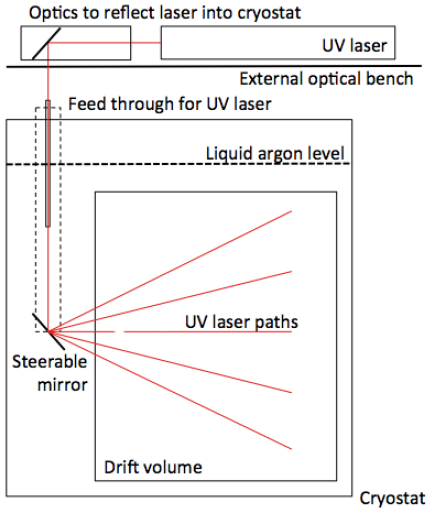
\includegraphics[width=0.45\linewidth]{uB_laser_schematic}
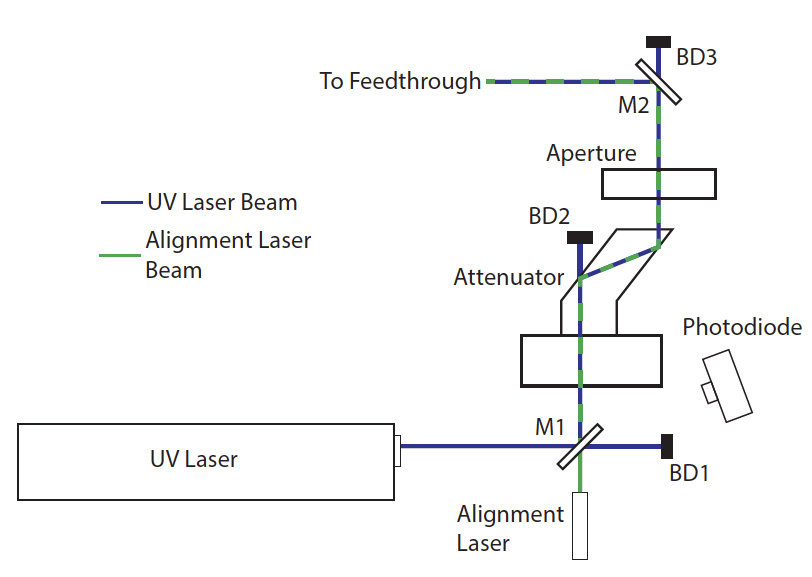
\includegraphics[width=0.5\linewidth]{uB_laser_box}
\end{dunefigure}

\begin{dunefigure}[\dshort{microboone} laser calibration system drawings]{fig:uB_laser_ft}
{CAD drawings of the \dword{microboone} laser calibration system~\cite{microboone}. Left: calibration port feedthrough. Right: laser beam periscope. %Both figures from~\cite{microboone}.
}
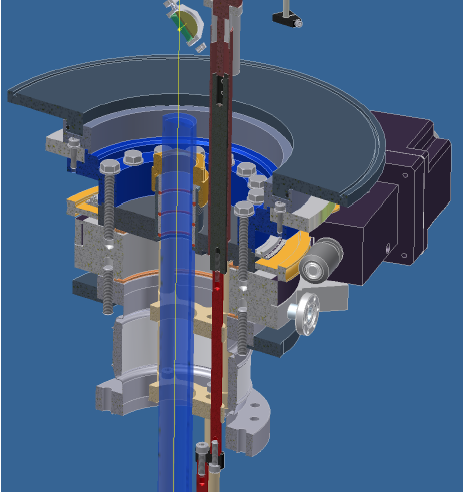
\includegraphics[width=0.49\linewidth]{uB_laser_ft}
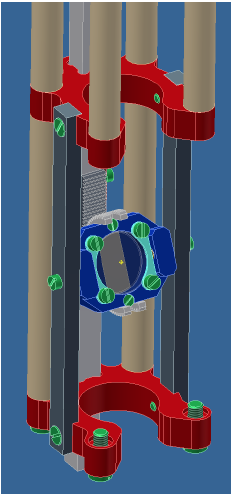
\includegraphics[width=0.248\linewidth]{uB_laser_periscope}
\end{dunefigure}

The goal of the mechanical design of the system is to achieve a precision close to that of the \dword{tpc} position measurements, so that no single factor dominates %in 
the overall systematics. The \dword{tpc} precision of about \SI{5}{\milli\m} in the $y$, $z$ coordinates is given primarily by the wire spacing of \uvpitch and \xgpitch. The precision of about \SI{2}{\milli\m} on the $x$ coordinate comes essentially from the \fepeaktime peaking time of the front-end electronics and the typical drift velocity (\driftvelocity).

The starting point of the laser beams is given by the position of the mirror in the periscope, which is known from construction drawings, warm surveys and cool down calculations. The angle of the beam is given by the angles ($\theta$, $\phi$) of the mirror, which are set by the periscope motors and read out by the encoders. 
For \dword{microboone}, reference~\cite{bib:chen2018} quotes a very good \SI{0.05}{\mrad} precision (\SI{0.5}{\milli\m} at \SI{10}{\m}) from the encoders alone, and an overall pointing precision of \SI{2}{\milli\m} at \SI{10}{\m}, driven mostly by beam size and divergence. In fact, with a \SI{0.5}{\mrad} divergence, we expect the beam to be \SI{5}{\milli\m} wide at \SI{10}{\m}.

In \dword{dune}, we aim to reach a similar precision. This will require a number of design and installation considerations: having encoders of similar high accuracy, carrying out surveys in various reference frames, and a capability to do location checks with a precision of about \SI{5}{\milli\m}  at \SI{20}{\m} from the beam origin. Therefore we aim to have a system that can locate the beam end point in few positions and attached to different references, at least one per drift volume and laser beam. 
%The goal of the laser system mechanical design and the laser location/positioning system is to achieve a precision close to that of the \dword{tpc} measurements, so that no single factor dominates the overall systematics.
%This corresponds to  providing the position of the beam to an accuracy of \SI{5}{\milli\m} with positioning systems located at about \SI{20}{\m} from the beam origin.
The independent laser beam location system is described in Section~\ref{sec:sp-calib-sys-las-loc}. 


\paragraph{Coverage estimations and top \dword{fc} penetration}
\label{sec:lasercoverage}

%\fixme{New sentences below. SG, please check and remove this.}
A crucial aspect of the design of the full array is the position of the periscope and the cold mirror with respect to the \dword{fc}, since its profiles can induce significant shadows and limit the beam's coverage. In order to address this aspect and motivate the design choices, we carried out a set of shadowing calculation studies.

Given that the \dword{fc} profiles are \SI{4.6}{\cm} wide with only a small \SI{1.4}{\cm} gap between them, the shadows produced if the laser source is located outside the \dword{fc} would be substantial. We estimate that the maximum angle at which beams can go through is about \ang{45}. Given the limitations of the region above the \dword{fc} (shown in Figure~\ref{fig:laser_topfc}, left), especially the geometry of the ground plane, it is likely that the mirror cannot be placed much higher up than \SI{40}{\cm} away from the \dword{fc}. 
With those assumptions, we have carried out a rough estimation of the fraction of voxels that would be crossed by any unblocked track. For simplicity, we are considering only a single vertical plane, so the coverage is actually overestimated since it does not consider the effect of the \dword{fc} I-beams, transverse to the \dword{fc} profiles.
Figure~\ref{fig:laser_topfc} (right) shows an example of those calculations. Assuming \SI{10}{\cm} voxels and no track directed at the \dword{apa}, the coverage is at most \SI{30}{\%}. Assuming \SI{30}{\cm} voxels and allowing all tracks directed at the \dword{apa}, the maximum coverage would be \SI{58}{\%}.

\begin{dunefigure}[View of top field cage and laser coverage estimation]{fig:laser_topfc}
{View of the top field cage (left) and laser 2D voxel coverage estimation for one drift volume (right).}
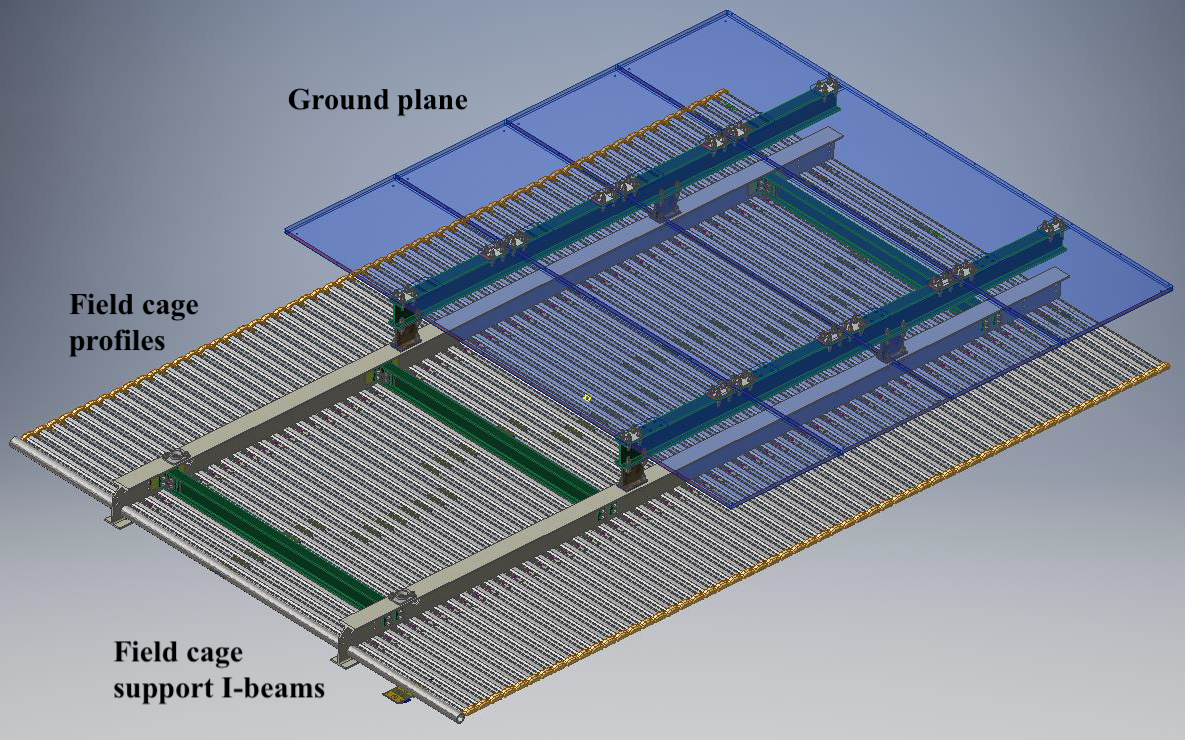
\includegraphics[width=0.7\linewidth]{calib-topFC_edit.png}
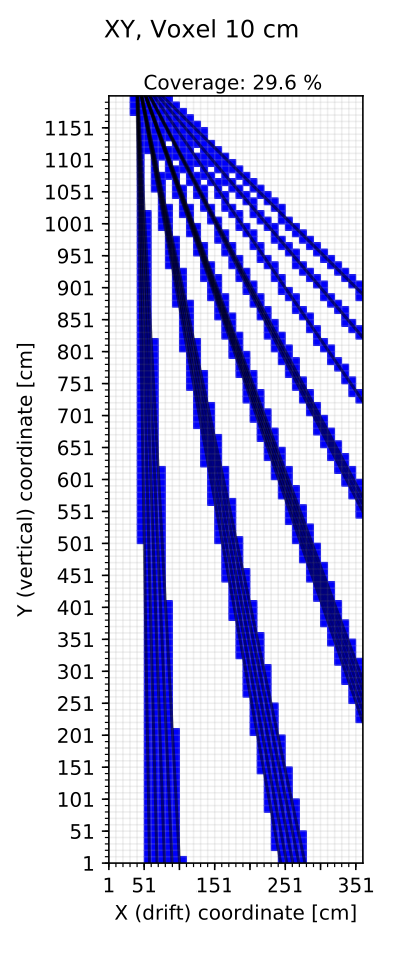
\includegraphics[width=0.29\linewidth]{calib-cov_XY_vox10_top_np1_noAPA_edit.png}
\end{dunefigure}

Penetration of the \dword{fc} would eliminate most of these shadows and allow for a practically unimpeded coverage. Depending on the depth of the periscope within the \dword{tpc}, some partial shadowing from the field cage support I-beam would still remain.
Figure~\ref{fig:laser_fcpenetration} shows a possible way to accomplish this for the top-of-TPC ports~\cite{bib:yu2019a}. A CAD model of the \dword{sbnd} laser calibration system periscope was used as 
%an example the design 
reference design for \dword{dune}. The \dword{sbnd} periscope, when rotating over its axis, requires a \SI{12}{\cm} diameter circular region free of impediments. In order to take into account a tolerance for the estimated \SI{0.3}{\%} shrinkage of the \dword{fc} at cryogenic temperatures, we chose an opening of three profiles, equivalent to \SI{18}{\cm}. 
%\fixme{New sentence below. SG, please check and remove this.}
Still, in order to minimize any risk associated with the presence of material close to the \dword{fc}, ongoing design studies will evaluate the feasibility of implementing vertically retractable periscopes, with a travel range sufficient for them to clear the top of the \dword{fc}. 

\begin{dunefigure}[Laser periscope penetrating the field cage]{fig:laser_fcpenetration}
{CAD drawing of one way the periscope could penetrate the \dword{fc}~\cite{bib:yu2019a}.}
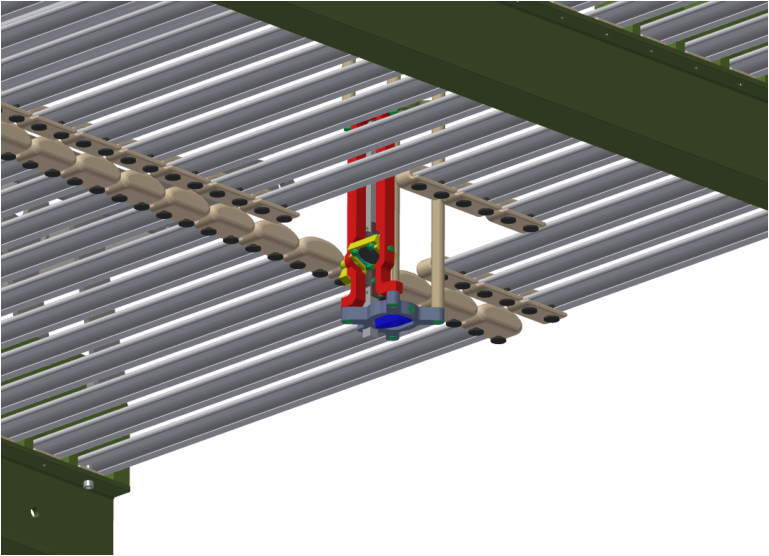
\includegraphics[width=0.6\linewidth]{laser_fcpenetration.pdf}
\end{dunefigure}

Simulations of the effect of \dword{fc} penetrations on the \efield were carried out~\cite{bib:yu2017b}, and are illustrated in Figure~\ref{fig:efield_penetration_boyu2017}. These have shown that the effect of a \SI{12x12}{\cm} opening (equivalent to two profiles), located at \SI{40}{\cm} (along the $x$ direction) from the \dword{apa}, is small and tolerable, with a maximum \SI{10}{\kilo\volt\per\cm} \efield caused by the opening and periscope.
These simulations need to be redone with a larger opening of \SI{18x18}{\cm}  (i.e., three profiles).
Still, if we were to choose, conservatively, to discard from the physics data analysis the volume within the \dword{tpc} determined by the periscope lateral size, a vertical penetration of \SI{10}{\cm}, and the full drift length (\SI{12x10x360}{\cm} = \SI{43}{\litre} for each of the \num{12} periscopes), it would represent only a very small fraction of \num{5e-6} of the full detector volume.

\begin{dunefigure}[Simulation of impact on \efield of \dshort{fc} penetration]{fig:efield_penetration_boyu2017}
{Simulation of the effect on the \efield of a laser periscope penetration of the \dword{fc}. In this case, an opening of only two profiles was considered.}
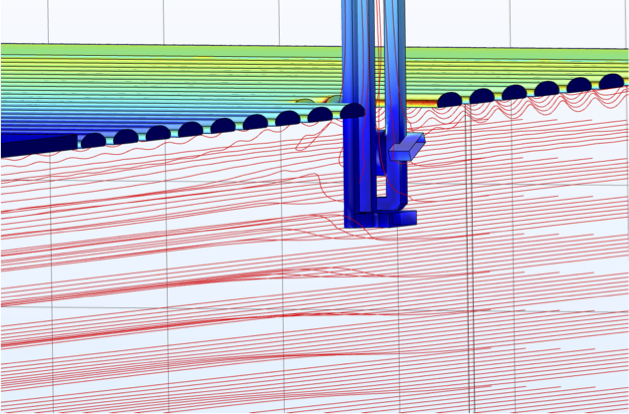
\includegraphics[width=0.6\linewidth]{efield_penetration_boyu2017.png}
\end{dunefigure}


\paragraph{Full array scope considerations}

As mentioned earlier (Section~\ref{sec:sp-calib-laser-req}), the system should allow for crossing laser beam tracks wherever possible. In order to %have 
collect them in the full \dword{spmod} volume, that would require using all the available \num{20} calibration ports. Since it is possible to use an iterative method to obtain displacement maps in regions where no crossing tracks are available, 
%for cost compromise reasons 
to minimize the overall cost of the system, the baseline design will use only the \num{12} central ports, providing crossing tracks in essentially \SI{50}{\%} of the detector volume. 
%Actually, 
In addition, for the six most central ports, close to the central \dword{apa}, the distance between them is small enough that we can consider having the same laser box serve two feedthroughs to reduce the costs associated with the laser and its optics. In that case, the total number of lasers needed would be nine.

Usage of the end-wall ports, which are not %over 
on top of the \dword{tpc}, is therefore not part of the baseline design, and is considered only as an alternative in Section~\ref{sec:sp-calib-laser-alter}. A coverage calculation for possible end-wall periscopes, taking into account the shadowing of both the \dword{fc} profiles and the support beams, gives a maximum of \SI{56}{\%} coverage for \SI{30}{\cm} voxels (allowing all tracks directed at the \dword{apa}). In this case the laser beams would enter the \dword{fc} laterally and \dword{fc} penetration would be harder to consider, so an alternative mechanical design aimed at improving the coverage, is considered in Section~\ref{sec:sp-calib-laser-alter}.



%a \SI{266}{\nano\m} laser would be mounted on the top of the cryostat, and service two adjacent feedthroughs. A steerable head and fiber interface would be mounted in the feedthrough, which is coated in a insulator. Two options are under investigation: (1) the \dword{fc} (but not the \dword{gp}) is penetrated, and (2) the \dword{fc} is not penetrated. In the former case, the \dword{fc} penetration has been shown to create a small distortion to the E-field, for the benefit of full volume E-field mapping. When the \dword{fc} is not penetrated, the laser shines through the \dword{fc} tubes, producing some regions that are not mappable by the laser. Unlike the ports that are inwards of the cryostat, the lasers through penetrations that are outside the \dword{fc} on the far east and west side of the cryostat will not penetrate the field cage. The photo-electron system would include a fiber and no steering; the necessity of penetrating the \dword{fc} is unlikely but has not been assessed yet.

A scan of the full detector using \num{10}$\times$\num{10}$\times$\SI{10}{\cubic\cm}
volume elements would require a number of tracks approximately \num{8e5} 
%would 
and can take about three days. Shorter runs could be done to investigate specific regions. The sampling granularity, and therefore the amount of data taken, depends on \dword{daq} requirements. In fact, even to be able to record the desired \num{8e5} tracks, a dedicated data reduction algorithm must be devised, so that only a drift window of about \SI{100}{\micro\s}
of data is recorded, and the position of that window depends on the beam position and direction and which wires are being read out. More details on this are given in Section~\ref{sec:sp-calib-daqreq}.

%The direct ionizing laser system may also be used to create \phel{}s from the cathode, even under low power operation.

%% JM %% end % from early IDR version




%%%%%%%%%%%%%%%
%\subsubsubsection{Possible Measurements}
\subsubsubsection{Measurement Program}
\label{sec:sp-calib-sys-las-ion-meas}

This section describes the methods used to measure 
%drift velocity and \efield 
parameter maps and their expected precision, given the design outlined above.

\paragraph{\efield and drift velocity measurement}
The method for \efield measurement is based on the measurement of apparent position displacements of the straight laser tracks. The laser produces straight tracks with a known starting position and direction. If, when reconstructed under the assumption of uniform and homogeneous drift velocity, any deviations from that are observed, they are attributed to \efield distortions. 

The first step in the analysis~\cite{bib:uBlaser2019} is to obtain a field of position displacements by comparing the known and reconstructed tracks. If two crossing tracks are used, the displacement vector is simply given by the vector connecting the point where the reconstructed tracks cross and the point where the known tracks cross. However, since those displacements can vary both in direction and magnitude, there will be ambiguity in that determination if only one track is used in a given spatial region. An iterative procedure was developed by the \dword{microboone} collaboration~\cite{bib:chen2018,bib:uBlaser2019} to obtain a displacement map from a set of several non-crossing tracks from opposite directions. Following this, a set of drift velocity field lines, which are the same as \efield lines, can be obtained from the displacement map, assuming that all charge deposits along a field line will be collected in the same position. Using the relationship between \efield and drift velocity~\cite{Li:2015rqa,Walkowiak:2000wf}, we can then also obtain the magnitude of the \efield.

Since the observed position distortion in one location depends on \efield distortions in many locations along the drift path, this method of analysis clearly requires the acquisition of data from many different tracks crossing each detector drift volume at many different angles. 

As already indicated in the previous section (section~\ref{sec:sp-calib-sys-las-ion-des}), the pointing precision will be on average \SI{2}{\milli\m} (at average distances of \SI{10}{\m}), and the \dword{tpc} precision is \SI{2}{\milli\m} in $x$ and \SI{5}{\milli\m} in $y$, $z$. Conservatively taking those in quadrature, we get $\sigma_x$ =  \SI{3}{\milli\m} and $\sigma_{yz}$ = \SI{5.4}{\milli\m}.
If we would use only one track per direction, in regions of size $l$ = \SI{300}{\milli\m}, we would therefore be sensitive to drift velocity field distortions of $\sigma /l$, i.e., \SI{1}{\%} in $x$ and \SI{1.8}{\%} in $y$, $z$. 

In order to estimate the \efield precision, we must distinguish between the $x$ and $y$, $z$ coordinates. To first order, distortion in $y$, $z$ do not affect the magnitude of the field, and so the relative distortions on \efield are equal to the relative distortions of the velocity. Along $x$, we must consider the relation between the magnitudes of the drift velocity and \efield. Using the formula from~\cite{Li:2015rqa,Walkowiak:2000wf} we can see that, at \spmaxfield, a \SI{1}{\%} change in \efield leads to a corresponding change of \SI{0.375}{\%} in drift velocity. We therefore reach the values of \SI{2.7}{\%} ($=1./0.375$) in $x$ and \SI{1.8}{\%} in $y$, $z$ for a conservative estimate of \efield precision using a single track per direction. 

This is a conservative estimate because it does not take into account the fact that the centroid of the beam should be known better than its full width, and because it is based on the assumption of a single track per direction.  
As observed in \dword{microboone}~\cite{bib:uBlaser2019}, using several tracks improves the precision, and in most of the volume an accuracy of \SI{1}{\%} was reached so the amount of statistics needed to reach \SI{1}{\%} will be an important question to address in the development plan. 






%The \dword{tpc} precision of about \SI{5}{\milli\m} in the $y$, $z$ coordinates is given primarily by the wire spacings of \uvpitch and \xgpitch.
%, and the 
%The precision of about \SI{2}{\milli\m} on the $x$ coordinate comes essentially from the \fepeaktime peaking time of the front-end electronics and the typical drift velocity (\driftvelocity).


%For distortions present in regions of \SI{0.5}{\m} and larger, drift velocity distortions can therefore be measured with an accuracy of \SI{1}{\%} in $y$, $z$ and \num{0.4}\% in $x$. 
%In $y$, $z$, \SI{1}{\%} precision on drift velocity distortions translates to a \SI{1}{\%} precision on the transverse field distortions. Along $x$, one must consider that, at \spmaxfield, a \SI{1}{\%} change in \efield leads to a \SI{0.375}{\%} change in drift velocity. Therefore, finally, this means that the smallest measurable distortions given the \dword{tpc} design (wire pitch, timing precision) are of \SI{1}{\%} in \efield if they are present in regions of \SI{0.5}{\m} and larger (smaller field distortions could, in principle, be measurable if they are present over larger regions, so that their effect accumulates over the drift path).

On one side, this gives us an ultimate limit to the \efield precision achievable with the laser system, but on the other side, since these \dword{tpc} precision considerations apply to physics events also, it tells us that an \efield precision much better than \SI{1}{\%} should not have an effect on the physics.

%\fixme{New paragraph. Needs checking. Probably needs also new references on lieftime measurements in ICARUS and uB}

\paragraph{Charge-based measurements}

Electron drift-lifetime~\cite{bib:uBlifetime, Antonello:2014eha} is the parameter that governs the dependence of the amount of collected charge on the drift time. A possible measurement of electron drift-lifetime would therefore require a very good control over the charge profile of the ionization laser tracks. This was achieved in a small scale experiment that measured lifetime with laser beams~\cite{Ereditato:2013xaa}, but is harder with longer distances. The charge produced by the laser tracks along its path depends on distance because the light intensity is reduced due to beam divergence and scattering, as well as non-linear effects such as the self-focusing, or Kerr effect. For this reason, the first steps in any laser-based charge measurement are a fine-tuning of the laser intensity in order to reduce self-focusing to a minimum, and ``charge profile calibration scan'' which consists of acquiring tracks parallel to the \dword{apa}. In order to get good statistical precision, several tracks could be acquired, in the same or different direction, but always parallel to the \dword{apa} in order to factorize out any effect from electron drift-lifetime. This set of data provides a calibrated laser beam charge profile that can then be used to analyse and normalize the measured charge profile from tracks that do have an angle with respect to the \dword{apa} and therefore span different drift times.

As for electron-ion recombination, since the $dE/dx$ for laser beams is much smaller than for charged particles, the effect should also be much smaller. However, that small effect has been observed~\cite{Badhrees:2010zz}, so a similar method than described above could be used to evaluate any dependence of the electron-ion recombination factor on the angle $\phi$ between the track and the electric field, that is predicted in some models~\cite{Acciarri:2013met}. This would entail taking data with tracks as parallel as possible to the \efield, in order to enhance the angular dependence term on the recombination expression (that goes with $1/sin \phi$), and to compensate for the smaller $dE/dx$ for laser beams.



